% This LaTeX was auto-generated from MATLAB code.
% To make changes, update the MATLAB code and export to LaTeX again.

\documentclass{article}

\usepackage[utf8]{inputenc}
\usepackage[T1]{fontenc}
\usepackage{lmodern}
\usepackage{graphicx}
\usepackage{color}
\usepackage{hyperref}
\usepackage{amsmath}
\usepackage{amsfonts}
\usepackage{epstopdf}
\usepackage[table]{xcolor}
\usepackage{matlab}

\sloppy
\epstopdfsetup{outdir=./}
\graphicspath{ {./EM_example_images/} }

\begin{document}

\matlabtitle{Gaussian Mixture: EM algorithm}

\begin{par}
\begin{flushleft}
1- Create the mixture
\end{flushleft}
\end{par}

\begin{matlabcode}
mu = [1; 9];
sigma = zeros(1,1,2);
sigma(1,1,1) = 0.5;
sigma(1,1,2) = 0.5;

x = linspace(-2,15,300)';
p1 = [0.3,0.7];

M1 = gmdistribution(mu,sigma,p1);
MM1 = M1.pdf(x);
\end{matlabcode}

\begin{par}
\begin{flushleft}
2- Sample the mixture
\end{flushleft}
\end{par}

\begin{matlabcode}
rng(3)
Y = random(M1,50)'
\end{matlabcode}
\begin{matlaboutput}
Y = 1x50    
    8.2075    9.8171    0.1442    8.8333    9.4084    9.0987    0.7269    1.0454   -0.1108    9.4905    0.9664    8.9080    9.1382    0.7465    7.3875    8.3064    1.4610    8.5940    1.5123    7.3018    1.5885    7.9239    7.9331    1.3259    9.0606    8.6797   10.1803    0.5893    9.3200    9.0754    9.4638    8.5299   10.3348    9.7996    9.7767    1.3619    8.9398    9.6193    9.7211    0.6352    9.5654   10.2435    1.2301    0.6117    9.2196    8.5399    9.1209    0.9323    0.2577    8.0402

\end{matlaboutput}

\begin{par}
\begin{flushleft}
3- See what we got
\end{flushleft}
\end{par}

\begin{matlabcode}
figure(1)
plot(x,MM1,'LineWidth',2,'Color',[1 0.2 0.2 1])
hold on
ylim([-0.1 0.3])
scatter(Y,zeros(size(Y)), 'xb')
\end{matlabcode}
\begin{center}
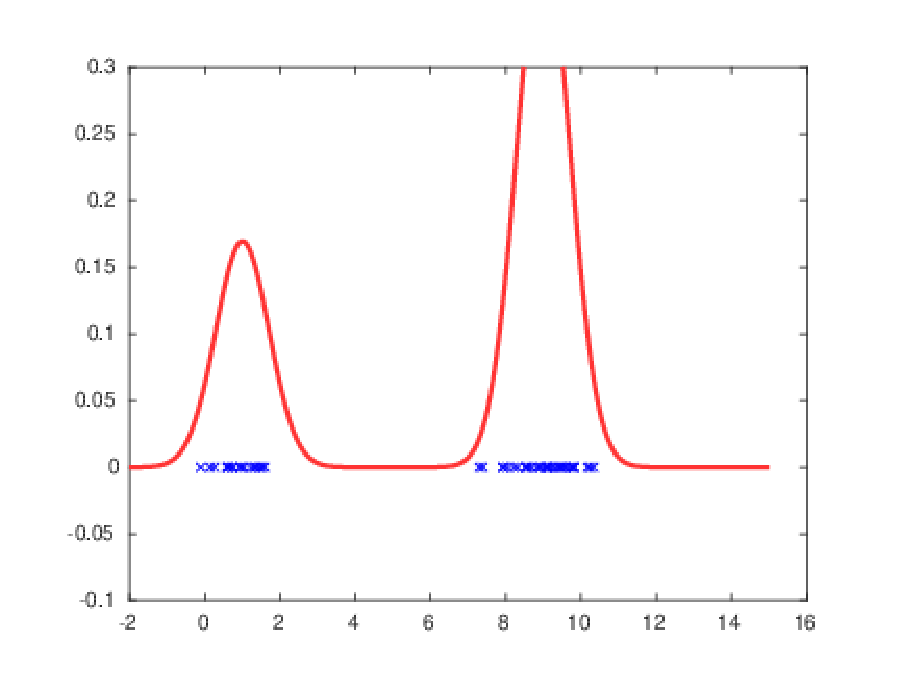
\includegraphics[width=\maxwidth{56.69844455594581em}]{figure_0.eps}
\end{center}

\begin{par}
\begin{flushleft}
4- Initialize variables. 
\end{flushleft}
\end{par}

\begin{matlabcode}
muhat = [4; 6];
sigmahat = zeros(1,1,2);
sigmahat(1,1,1) = 1;
sigmahat(1,1,2) = 1;
phat = [0.5 0.5]
\end{matlabcode}
\begin{matlaboutput}
phat = 1x2    
    0.5000    0.5000

\end{matlaboutput}


\begin{par}
\begin{flushleft}
5- Iterate the E-step and M-step (see functions below)
\end{flushleft}
\end{par}

\begin{matlabcode}
niter = 6;
rem = 3;

figure(2)

subplot(niter/rem + 1, 1, 1)
Mhat = gmdistribution(muhat,sigmahat,phat);
MMhat = Mhat.pdf(x);
plot(x,MM1,'LineWidth',2,'Color',[1 0.8 0.9 1])
hold on
plot(x,MMhat, 'LineWidth', 2, 'Color', [0.8 0.8 1 1])
legend('Real mixture','Estimated mixture')
hold off

for i=1:niter
    g = e_step(Y,muhat,sigmahat,phat);
    [muhat,sigmahat,phat] = m_step(g,Y);

    Mhat = gmdistribution(muhat,sigmahat,phat);
    MMhat = Mhat.pdf(x);
    
    if mod(i,rem) == 0
        subplot(niter/rem+1,1,i/rem+1)
        plot(x,MM1,'LineWidth',2,'Color',[1 0.8 0.9 1])
        hold on
        plot(x,MMhat, 'LineWidth', 2, 'Color', [0.8 0.8 1 1])
        legend('Real mixture','Estimated mixture')
        hold off
    end
end
\end{matlabcode}
\begin{center}
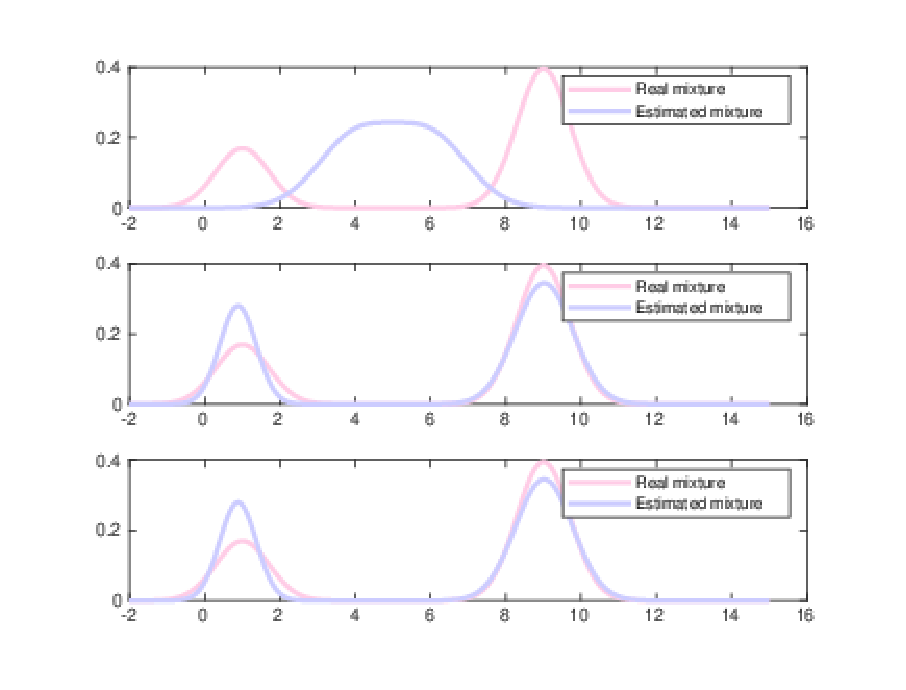
\includegraphics[width=\maxwidth{56.69844455594581em}]{figure_1.eps}
\end{center}
\begin{matlabcode}
muhat
\end{matlabcode}
\begin{matlaboutput}
muhat = 2x1    
    0.8838
    9.0175

\end{matlaboutput}
\begin{matlabcode}
sigmahat(1,1,:)
\end{matlabcode}
\begin{matlaboutput}
ans = 
ans(:,:,1) =

    0.2352


ans(:,:,2) =

    0.5825

\end{matlaboutput}
\begin{matlabcode}
phat
\end{matlabcode}
\begin{matlaboutput}
phat = 1x2    
    0.3400    0.6600

\end{matlaboutput}


\begin{matlabcode}
function g = e_step(Y,muhat,sigmahat,pihat)
    g = zeros(length(Y),length(muhat));
    denom = zeros(length(Y),1);
    for k=1:length(muhat)
        g(:,k) = pihat(k)*normpdf(Y(:),muhat(k),sigmahat(1,1,k));
        denom = denom + pihat(k)*normpdf(Y(:),muhat(k),sigmahat(1,1,k));
    end
    g = g./denom;
end

function [muhat,sigmahat,pihat] = m_step(g,Y)
    s = size(g);
    muhat = zeros(s(2),1);
    for k=1:s(2)
        muhat(k) = Y*g(:,k) / sum(g(:,k));
    end

    sigmahat = zeros(1,1,s(2));
    for k=1:s(2)
        sigmahat(1,1,k) = (Y-muhat(k)).^2*g(:,k) / sum(g(:,k));
    end

    pihat = zeros(1,s(2));
    for k=1:s(2)
        pihat(k) = sum(g(:,k)) / length(Y);
    end
end
\end{matlabcode}

\end{document}
